\documentclass{beamer}
\usepackage[english,russian]{babel}

\usepackage{graphicx}

%\usepackage{xcolor}
%\usepackage{hyperref}


\usetheme{Berlin}
\usecolortheme{spruce}

% тип документа
% далее идёт преамбула
\title{Отчет по: Учебной ознакомительной практике}
\author{Автор: Усмонов Отабек}
\institute{группа:5-205.1}
\date{напишешь дату}
\begin{document}% начало презентации

\begin{frame}% первый слайд
\titlepage
\end{frame}
\section{Краткое введение в содержание всей практики}

\begin{frame}% второй слайд
\frametitle{Введение}


    
\end{frame}

\begin{frame}{Название слайда}
    \begin{columns}[T]
        \begin{column}{0.5\textwidth}
            если понадобится вставить текст
        \end{column}
        \begin{column}{0.5\textwidth} 
            
\includegraphics[width=\textwidth]{images/Fdp.png}
        \end{column}
    \end{columns}
\end{frame}

\begin{frame}{Название слайда}
    \begin{columns}[T]
        \begin{column}{0.5\textwidth}
           если понадобится вставить текст
        \end{column}
        \begin{column}{0.5\textwidth} 
            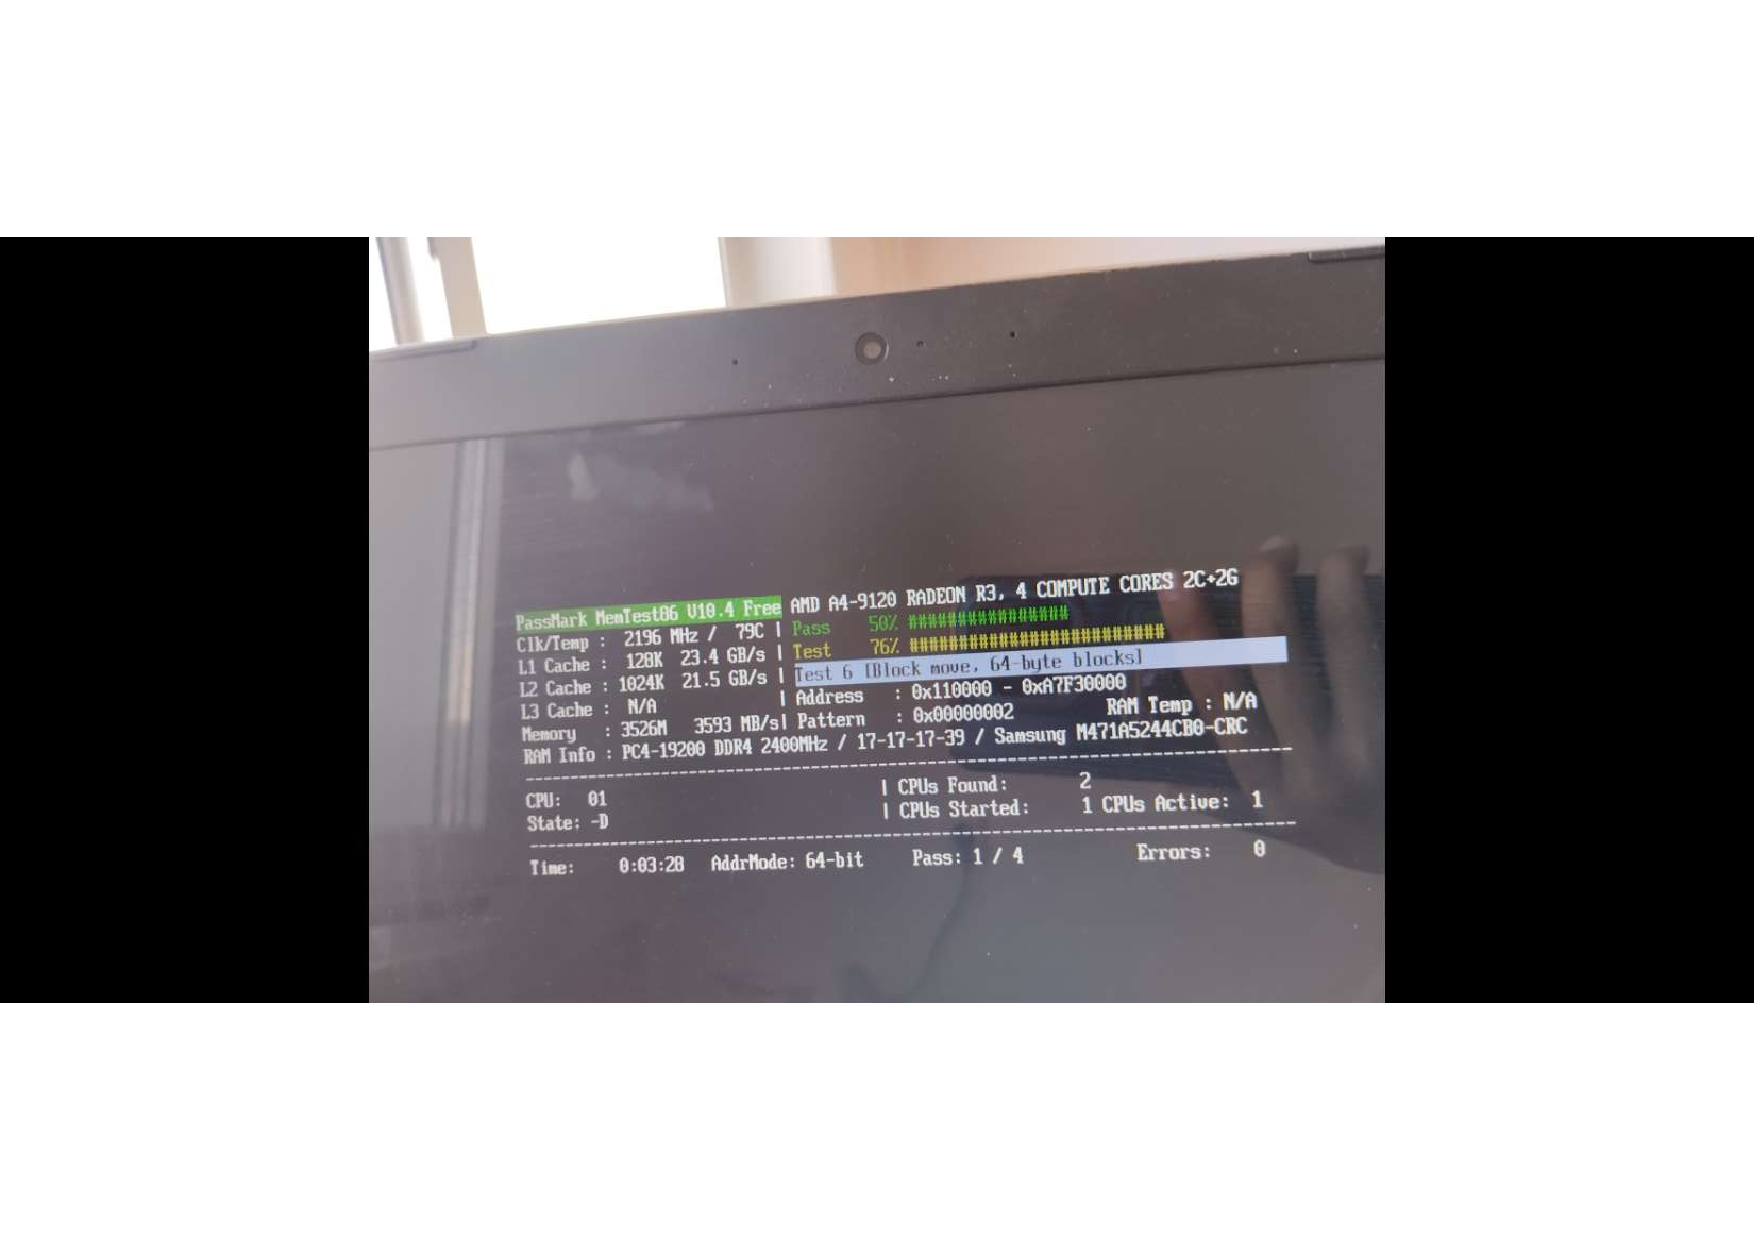
\includegraphics[width=\textwidth]{images/MemTest.pdf}
            %\caption{Запуск MemTest во время практики}
        \end{column}
    \end{columns}
\end{frame}
\begin{frame}{Название слайда}
    если понадобится вставить текст
\end{frame}
\begin{frame}{Название слайда}
    если нужно что-то перечислить
   \begin{itemize}
       \item Тест № 0
        \item Тест № 1 
        \item Тест № 2 
        \item Тест № 3  
   \end{itemize}
\end{frame}

\begin{frame}{Название слайда}
    \begin{columns}[T]
        \begin{column}{0.6\textwidth}
        если понадобится вставить текст
        \end{column}
        \begin{column}{0.4\textwidth}
            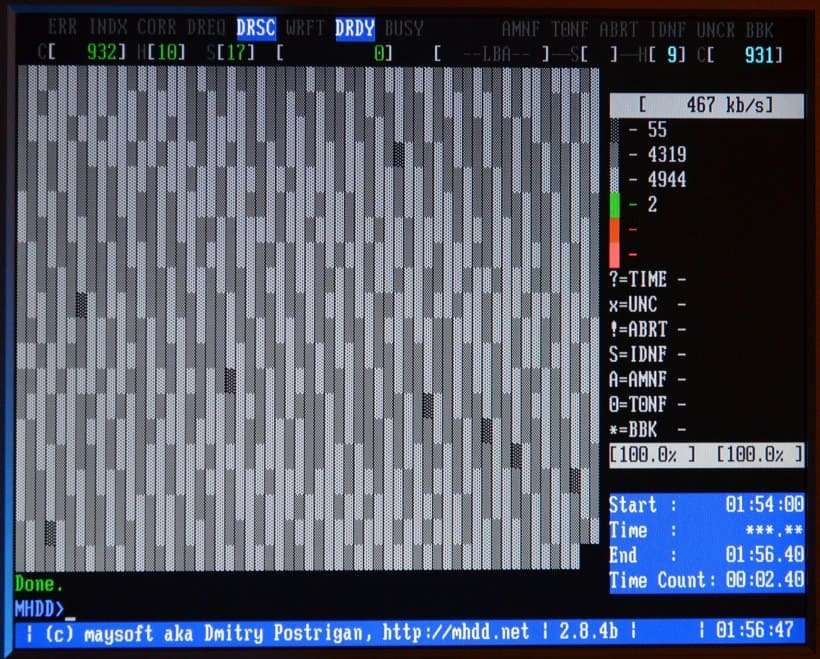
\includegraphics[width=\textwidth]{images/MHDD.jpeg}
        \end{column}
    \end{columns}
\end{frame}
\begin{frame}{Название слайда}
    \begin{columns}
        \begin{column}{0.6\textwidth}
            если понадобится вставить текст
        \end{column}
        \begin{column}{0.4\textwidth}
            
\includegraphics[width=\textwidth]{images/mhdd.png}
        \end{column}
    \end{columns}
\end{frame}
\begin{frame}{Название слайда}
если нужно что-то перечислить
    \begin{itemize}
        \item диагностика жесткого диска.
        \item Управление системой SMART жесткого диска.
        \item Возможность парольной защиты.
        \item Изменение звуковых характеристик винчестера.
        \item Изменение размера накопителя.
        \item Восстановление и низкое форматирование поверхности жесткого диска
    \end{itemize}
\end{frame}
\begin{frame}{Заключение}
можно не добавлять текст и закончить на этом
    \begin{center}
        \Huge{Спасибо за внимание!!!}
    \end{center}
\end{frame}

\end{document}